%%%%%%%%%%%%%%%%%%%%%%%%%%%%%%%%%%%%%%%%%
% UNSW School of Physics
% LaTeX Assignment Template
% Version 1.0 (Updated 21/02/17)
% Last update by Adam Micolich
%%%%%%%%%%%%%%%%%%%%%%%%%%%%%%%%%%%%%%%%%

% Packages and other configurations for document

\documentclass[paper=a4, fontsize=12pt]{scrartcl}

\usepackage{url}

\usepackage{hyperref}
\usepackage{graphicx}

\usepackage[T1]{fontenc} % Use 8-bit encoding that has 256 glyphs
\usepackage{fourier} % Use the Adobe Utopia font for the document - comment this line to return to the LaTeX default
\usepackage[english]{babel} % English language/hyphenation
\usepackage{amsmath,amsfonts,amsthm} % Math packages
\usepackage{graphicx} % Graphics packages
\usepackage{enumitem} % Lettered List Package
\usepackage{tikz} % Diagram Package
\usepackage{xcolor} % Colour Package
\usepackage{bm} % Bold Maths
\usepackage{caption} % Table titles

\usepackage{listings} % Code formatting
\usepackage{color}
 
\definecolor{codegreen}{rgb}{0,0.6,0}
\definecolor{codegray}{rgb}{0.5,0.5,0.5}
\definecolor{codeorange}{rgb}{0.7,0.2,0}
\definecolor{codered}{rgb}{0.7,0,0}
\definecolor{backcolour}{rgb}{0.95,0.95,0.92}
 
\lstdefinestyle{mystyle}{
    backgroundcolor=\color{backcolour},   
    commentstyle=\color{codered},
    keywordstyle=\color{codeorange},
    numberstyle=\tiny\color{codegray},
    stringstyle=\color{codegreen},
    basicstyle=\footnotesize,
    breakatwhitespace=false,         
    breaklines=true,                 
    captionpos=b,                    
    keepspaces=true,                 
    numbers=left,                    
    numbersep=5pt,                  
    showspaces=false,                
    showstringspaces=false,
    showtabs=false,                  
    tabsize=2
}
 
\lstset{style=mystyle}

% Block below sets up headers and sectioning.
\usepackage{fancyhdr} % Custom headers and footers
\pagestyle{fancy} % Makes all pages in the document conform to the custom headers and footers
\fancyhead[L]{z5173159 Cecilia Xifei Ni} %Page header left -- Student number and name
\fancyhead[C] {} %Page header center -- Empty
\fancyhead[R]{Word Embedding and Question Answering} %Page header right -- Course/year
\fancyfoot[L]{} % Empty left footer
\fancyfoot[C]{\thepage} % center footer -- page numbering
\fancyfoot[R]{} % Empty right footer
\renewcommand{\headrulewidth}{0pt} % Remove header underlines
\renewcommand{\footrulewidth}{0pt} % Remove footer underlines
\setlength{\headheight}{12pt} % Customize the height of the header
%\numberwithin{equation}{section} % Number equations within sections (i.e. 1.1, 1.2, 2.1, 2.2 instead of 1, 2, 3, 4)
%\numberwithin{figure}{section} % Number figures within sections (i.e. 1.1, 1.2, 2.1, 2.2 instead of 1, 2, 3, 4)
%\numberwithin{table}{section} % Number tables within sections (i.e. 1.1, 1.2, 2.1, 2.2 instead of 1, 2, 3, 4)
%\setlength\parindent{0pt} % Removes all indentation from paragraphs - comment this line for an assignment with lots of text

\usepackage{sectsty} % Allows customizing section commands
\allsectionsfont{\normalfont\scshape} % Make all sections default font with small caps
\renewcommand\thesection{} % Stops from putting section numbers in section headers but keeps numbering working.
\renewcommand\thesubsection{} % Stops from putting section numbers in section headers but keeps numbering working.
\renewcommand\thesubsubsection{} % See above

\usepackage{lipsum} % Inserts dummy latin text into template -- Can remove from final submission

% Title block on first page

\newcommand{\horrule}[1]{\rule{\linewidth}{#1}} % Create horizontal rule command with 1 argument of height

\title{	\normalfont \normalsize
\textsc{UNSW School of Computer Science and Engineering} \\ [24pt]
\horrule{1pt} \\[0.5cm] % Thin top horizontal rule
\LARGE Word Embedding and Question Answering \\ % The assignment title
\horrule{1pt} \\[0.5cm] % Thick bottom horizontal rule
}

\author{Cecilia Xifei Ni z5173159} % Your name

\date{\normalsize\today} % Today's date or a custom date

\begin{document}\thispagestyle{empty}

\maketitle % Print the title
\section{Introduction}
\begin{figure}
  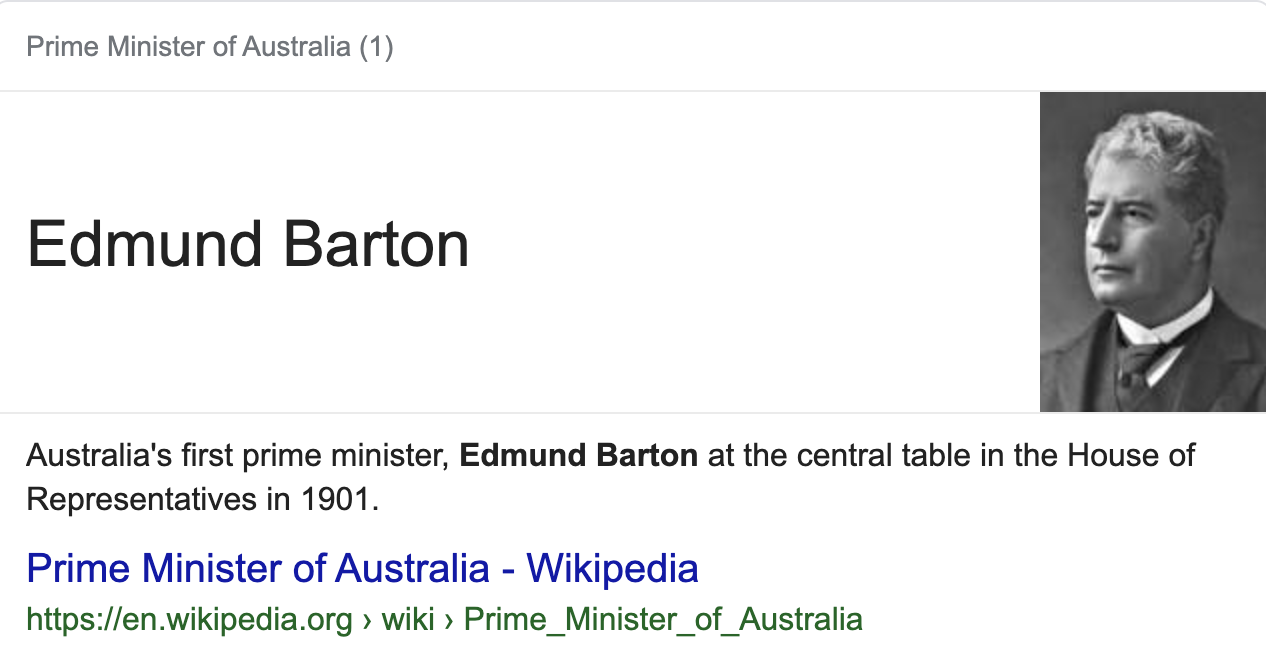
\includegraphics[width=\linewidth]{google.png}
  \caption{A result returned by Google to answer "Who is the first Prime Minister of Australia?"}
  \label{fig:google}
\end{figure}
"Who is the first Prime Minister of Australia?" \\\\
%% insert image
Figure 1 is a screen shot of search result returning by Google. This is a question a Question Answering (QA) system should be able to respond to. QA system evaluates texts across the web or database to find answer of a particular question to return in a form of short text.\\\\
Current machine algorithms extracts answer from a short paragraph instead of a long content (e.g. an entire wiki page/a news article). When applying modern machine learning algorithms on a long content, the result can be complicated and lenthy. \\\\
This essay aims to firstly gives a mathematical heavy explanation on nowadays natural language processing (NLP) algorithms, then propose my own heuristics based on them to predict answers from a long content based on the question being asked. \\\\
My algorithm will be tested with \href{https://ai.google.com/research/NaturalQuestions/dataset}{Google Natural Questions} which contains its own private testing dataset. 
\section{General Word Embedding Models}
\textbf{Word Embedding} is the collective name for techniques in NLP  where words or phrases are mapped into vectors of real numbers. \\\\
As per all machine learning algorithms, the general philosophy is to find the minimum of a converged function. When trying to convert words to number, its original utf code will not work well. What we need is a hard-coded map between the word itself, and its semantics. As human, we learn these semantics from daily experience which machine has no way to access, therefore, we need a mapping from words and its semantic in order for machine to decode.
\subsection{First Attempt: Hot One Encoding}
Given a collection of $N$ unique words, each word is of size $N$. The vector is very sparse such that only one index is 1 and others are 0. This is to say each word is a \textbf{dimension}. \\\\
\begin{figure}
  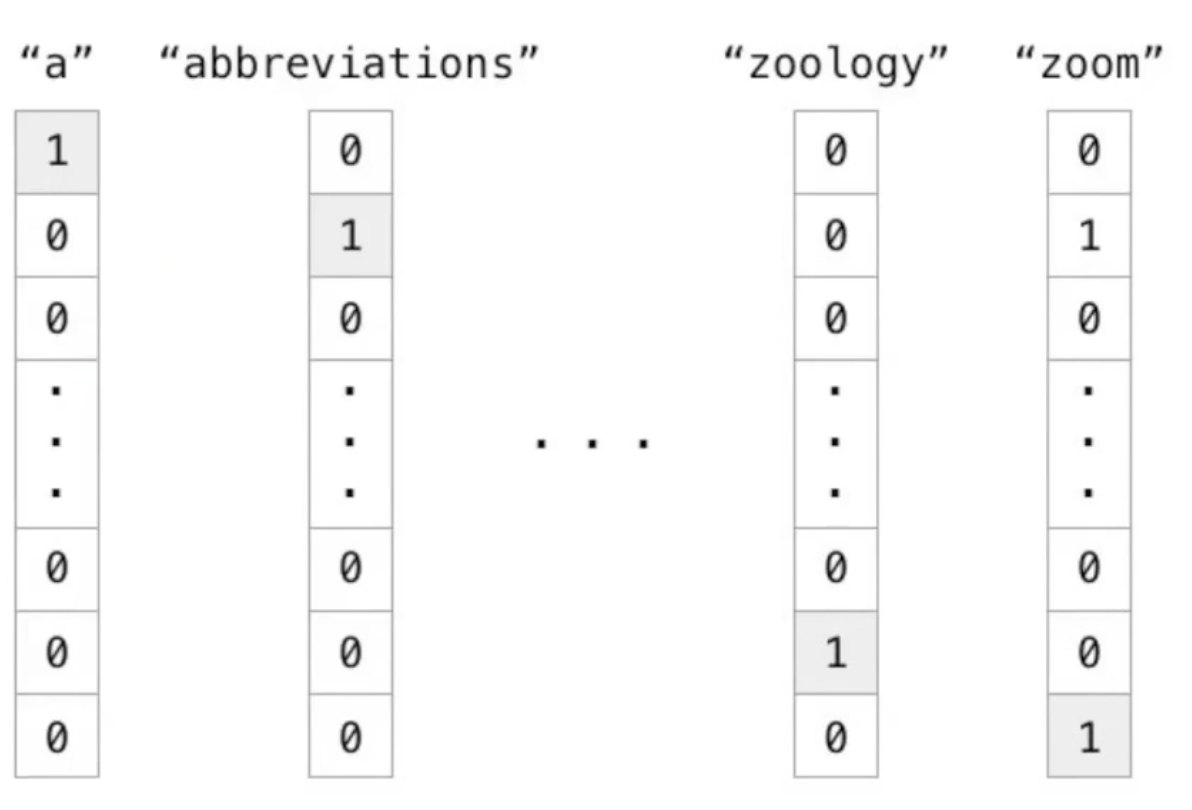
\includegraphics[width=\linewidth]{vectors.png}
  \caption{One Hot Encoding Example.}
  \label{fig:vector}
\end{figure}
Figure \ref{fig:vector} shows an example of hot encoding. \\\\
However, this model has some significant drawbacks. Firstly, it probably works fine for English as it has roughly 8000 frequent words. However, for languages like Chinese or Japanese, they are character-based, and each character will generate tons of combinations. This model will suffer from dramatic increase in dimensionalities. Secondly, all vectors in the matrix are independent to each other, while we do want them to learn the inter-connections between them.

\subsection{Second Attempt: Bag of Words (BoW) Model}
 On the second attempt, we focus more on extracting information from the perspective of the whole document. Under this model, we represent words in a document as a bag (multiset) of words-- we discard order and grammar, and only keep its multiplicity.\\\\
Here is an example:\\
Document 1: "George" "likes" "to" "play" "video" "games", "Mary" "likes" "video" "games" "too".\\
Document 2: "Mary" "also" "likes" "movies".\\\\
The BoW representation of the two above documentations is\\\\
BoW1: \{"George" : 1, "likes : 2", "to" : 1, "play " : 2, "video" : 2, "games" : 2, "Mary" : 1,  "too": 1\}\\
BoW2: \{"Mary" : 1, "also" : 1, "likes": 1, "movie" : 1\}\\
Here, each key is the word, and the value corresponds to occurrence. \\
\begin{figure}
  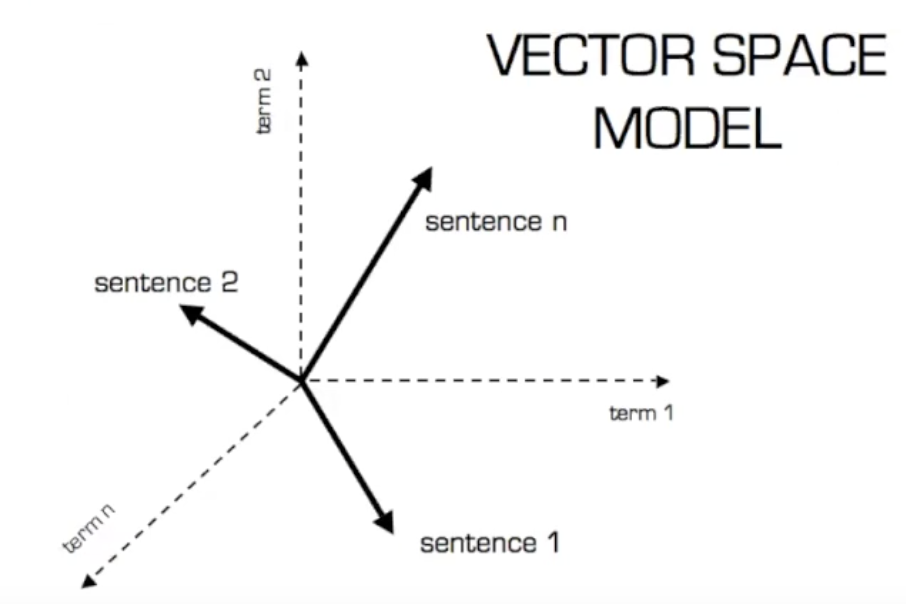
\includegraphics[width=\linewidth]{bow.png}
  \caption{Bag of Words Vector Space Representation}
  \label{fig:bow}
\end{figure}
This approach could be potentially used to compare similarities between two documents. When comparing them, we construct two vectors with each index corresponding to each unique words. Each be the count of the word appeared in that specific document. 
% more on cosine similarities/ euclidean distance.
The similarities of two documents can be measured by its Euclidean distance or its consine similarities. \\\\
Intuitively, two documents are similar if their vector points to the similar direction. We define the cosine similarities of two documents as: \\
\begin{align}
cosim(U_k, U_i) = \frac{\langle U_k, U_i \rangle}{\lVert U_k \rVert \cdot \lVert U_i \rVert}
\end{align}
where $\langle U_k, U_i \rangle$ is the scalar product of $U_i$ and $U_k$. 

\subsection{Third Attempt: Neural Network Based (NNLM)}
One intuitive question to ask is, Bag of Words and One Hot Encoding both treat each words as a separate dimension, but do we need so many dimensions?\\\\
The answer is probably no. Because a lot of words are similar or related. e.g. \\\\
Nouns: dog, cat, pet.\\
Verbs: fish, fished, fishing. \\
Adjective: very, great, significant. \\
Context: play {guitar, piano, games, tennis}\\\\
To not feel overwhelmed by the math at first, let's start with a easy example: \\
Words to be processed: boy, girl, woman, man \\
We can simply divide these words into two dimensions: gender and age as per Table 1 shows. This method is called \textbf{Distributed Representation}.\\\\
However, human language are so complex that we are not able to pre-define all dimensions for all words. Therefore we want to train a function $\mathbf{f}$ to get the word embedding for us. Figure 4 shows the function mapping. \\\\
To the best of my knowledge, we can do this in two ways. 
\begin{table}[]
\begin{tabular}{|l|l|l|}
\hline
       & 0     & 1      \\ \hline
gender & male  & female \\ \hline
age    & child & adult  \\ \hline
\end{tabular}
\caption{Table 1: Represent Words in Fewer Dimensions}
\end{table}

\begin{figure}
  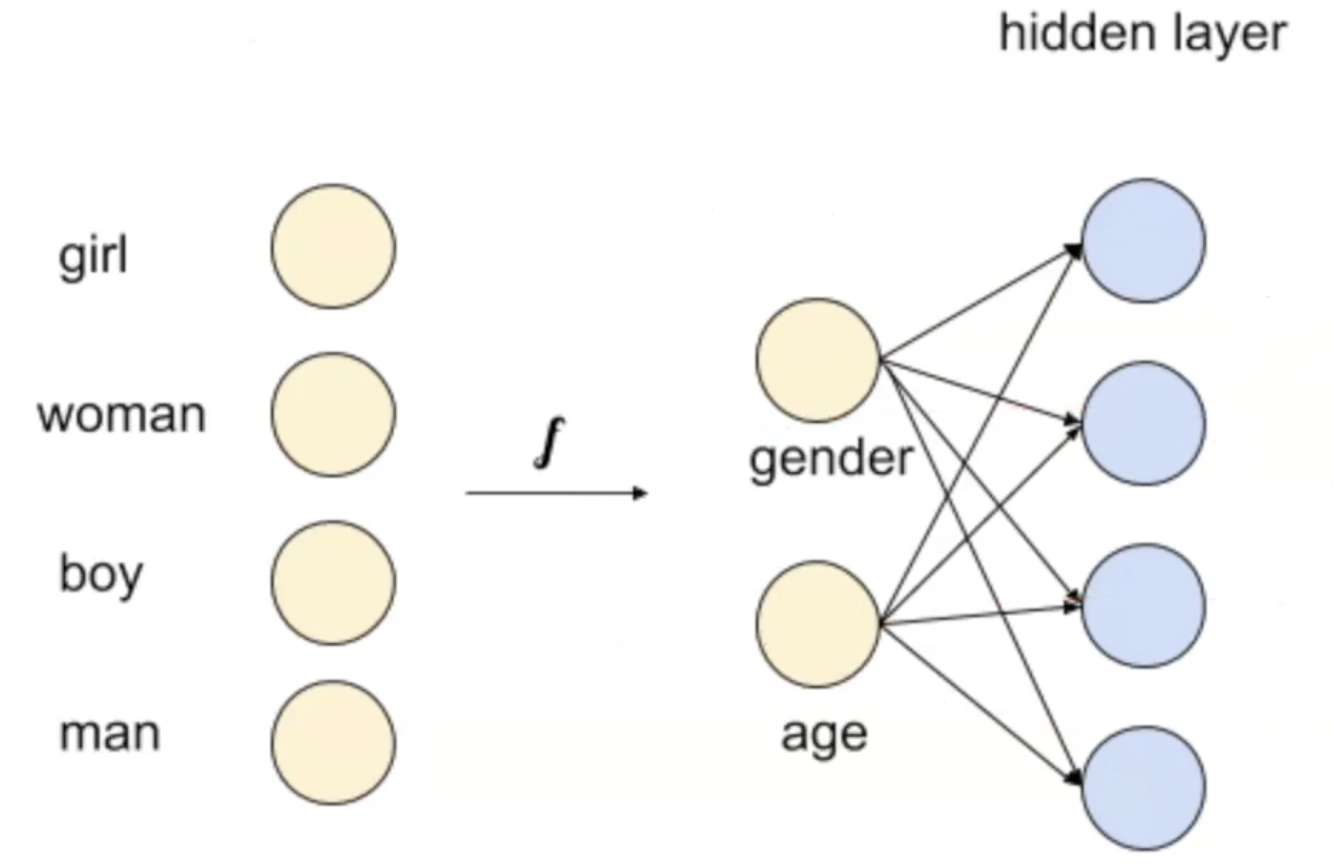
\includegraphics[width=\linewidth]{nnlm.png}
  \caption{Figure 4: Neural Network Based Mapping}
  \label{fig:nnlm}
\end{figure}
\subsubsection{Autoencoder (GAN)}
An autoencoder is a type of neural network that learns to label dimensions in an unsupervised manner. Figure 5 shows that an autoencoder is composed of two parts: the input side, marked as $X$, and the reconstruction (output) side, marked as $X'$. The $X$ tries to learn a distributed representation of the original data that aims to reduce the dimensions, and the $X'$ side is where the autoencoder tries to generate from the reduced representation as close as possible to its original input, hence its name, reconstruction. 
\begin{figure}
  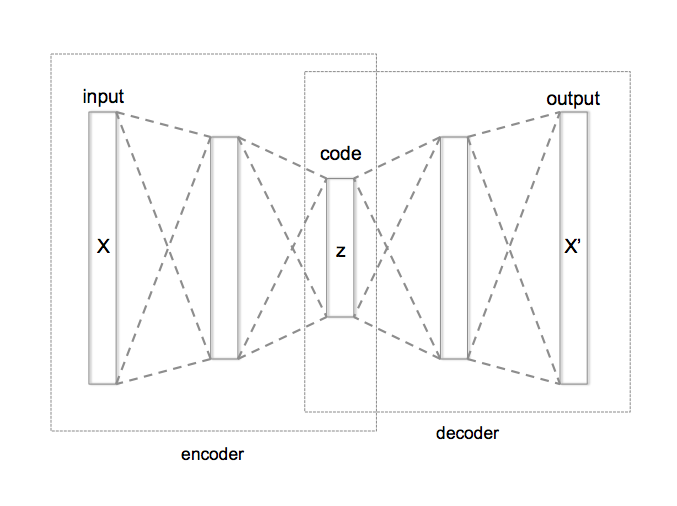
\includegraphics[width=\linewidth]{Autoencoder_structure.png}
  \caption{Figure 5: Schematic structure of an autoencoder with 3 fully connected hidden layers. The code (z, or h for reference in the text) is the most internal layer.}
  \label{fig:autoencoder}
\end{figure}
\paragraph{Basic Architecture of Autoencoder}
An autoencoder consists of two parts, the encoder and the decoder, which can be defined as transitions $\psi$ and $\phi$, such that:
\begin{align*}
& \psi : \chi \mapsto \mathfrak{F} \\
& \phi : \mathfrak{F} \mapsto \chi \\
& \psi, \phi = arg_{\psi, \phi} min \lvert \chi - (\psi * \phi) \chi \rvert
\end{align*}
In the simplest form, we assume there is only one hidden layer. The encoder stage of the autoencoder takes input $x \in \mathbb{R}^{d} = \chi$ and maps it to $\mathbf{h} \in \mathbb{R}^{p} = \mathfrak{F}$. \\
\begin{align*}
\mathbf{h} = \delta (\mathbf{W}x + \mathbf{b})
\end{align*}
This image $\mathbf{h}$ is the code section shown in Figure 5. $\delta$ is normally a sigmoid function defined as following: \\
\begin{align*}
S(x) = \frac{1}{1 + e^{-x}} = \frac{e^x}{e^x + 1}
\end{align*}
$\mathbf{W}$ is a weight matrix and $\mathbf{b}$ is a bias vector. The initializations of these two variables are random. They will be learnt iteratively through \textbf{backpropagation}. \\
\begin{align*}
\mathbf{h'} = \sigma (\mathbf{W'}x + \mathbf{b'})
\end{align*}
The backpropagation computes weight space $\mathbf{W}$ and bias vector $b$ with respect of a loss function $\mathbb{C}$.\\\\
$x$ : input (vector of features). \\
$x'$ : target output, the closer to $x$, the better. \\
$\mathbb{C}$: loss function, which intuitively associate with the "cost" of certain event or representation. The aim of training is to minimize the loss function. \\
$L$: the number of layers. In the above example, L equals to 1. However, here we aims to provide a generalized form.\\
$W^l = W^l_{j_k}$: the weights between layer  $l-1$ and $l$, where $W^l_{j_k}$ is the weight between the k-th node in layer $l$-1 and the $j$-th node in layer $l$.\\
$f^l$: sigmoid function at layer $l$.\\
The whole neural network can be represented by this function:\\
\begin{align*}
g(x) = f^{L}(W^Lf^{L-1}(W^{L-1}...f^1(W^1*x)...)
\end{align*}
For each input $x_i$, there will be an output $x'_i$ corresponding with it. the loss of the model on that pair is the cost of the difference between the predicted output $g(x_i)$  and the target output $x'_i$:\\
\begin{align*}
\mathbb{C}(y_i, f^{L}(W^Lf^{L-1}(W^{L-1}...f^1(W^1*x)...))
\end{align*}
For each layer, we compute the minimum of the loss function by calculating its derivatives. 
\begin{align*}
\frac{\partial \mathbb{C}}{\partial W^l_{j_k}}
\end{align*}
Where the loss function is defined as: 
\begin{align*}
\mathbb{C}(x, x') = \lvert x - x'\rvert^2 = \lvert x - \sigma'(\mathbf{W}'(\sigma (\mathbf{W}x + b)) + b' \rvert
\end{align*}
where $x$ is the average across all inputs.
\subsubsection{Neural Network Language Model (NNLM)}

\subsection{Fourth Attempt: Non-NN Model}






\clearpage

\begin{thebibliography}{99}
\bibitem{Lectures} Prof. Mike Gal, "Physical waves", Lectures, {\em UNSW: PHYS1241}
\bibitem{Workfunctions} R Nave, ''Work Functions for Photoelectric Effect'' {\em Hyperphysics} (2017), found at <http://hyperphysics.phy-astr.gsu.edu/hbase/Tables/photoelec.html>, accessed 26 Oct. 2017

\end{thebibliography}



\end{document} 